\documentclass{article}

%Margins
\usepackage[margin=1in]{geometry}
 
%Float & Graphics 
\usepackage{float}
\usepackage{graphicx}

%Chemistry Equations
\usepackage [version = 3] {mhchem}
\usepackage{chemmacros}

%Document
\begin{document}

%Insert Title Here 

\section*{Abstract}

\section*{Introduction} %Introduction
\subsection*{Purpose}
The purpose of this experiment was to determine the extent to which the pH of a 150 mL buffer solution between Acetic Acid, \ce{C_2H_4O_2}, and Sodium Acetate, \ce{C_2H_3NaO_2}, varied with temperature. 

\section*{Background}%Background
%pH
The pH of a solution is a measure of the molar concentration of hydrogen ions in the solution; threby, being a measure of the acidity or basicity of the solution. A pH of less than 7 is basic, greater than 7 is acidic, and 7.0 is neutral. The pH of a solution can be mathematically represented as the negative logarathim of the Molar concentration of the hydrogen ions present in solution, as shown below. 
\begin{eqnarray*}
pH = -\log_{10}[H^+]
\end{eqnarray*} \\
\noindent
The pH of a solution essentially states the extent of the veracity of an acid or base. The closer the pH of an acid is to 1, the stronger and more volatile the acid. Conversely, the closer the pH of a base is to 14, the stronger and more volatile the base. \\
\noindent
The pH of a solution is also known to vary by temperature. In a study conducted by Ashton and Geary, it was found that the pH of a solution varied by temperature, depending on the initial measured pH at room temperature, as shown in the table below. 
\begin{figure}[H]
	\centering
	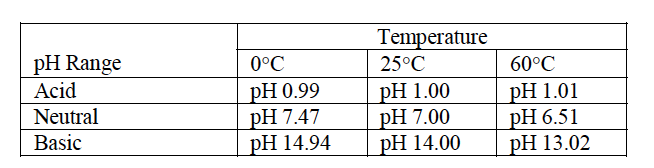
\includegraphics{/Users/abhisreekanth/Desktop/ChemHL-IA/Figures/1.png}
	\caption{Relationship of pH and temperature (2005, Ashton and Geary).}
\end{figure} 
\noindent
The pH of a solution varies with concentration as well. There is a linear relationship between the concentration of a solution and its subsequent pH. This is because the pH of a solution is the measure of the hydrogen ion concentration of the solution. For every increase in pH by a factor of 1, the concentration increases by a factor of ten. \\
\noindent
%pKa & 
The acid dissociation constant, $K_a$, is the measure of the strength of an acid in solution. The $K_a$ is found by solving the expression for the following acid dissocation reaction: \\

\begin{eqnarray*}
\ce{ HA_{\aq} <=> H^{+}_{\aq} + A^{-}_{\aq} }
\end{eqnarray*}

\noindent
Where HA is the generic acid, $H^+$ is the hydrogen ion, and $A^-$ is the conjugate base of the acid. The above reaction is in equilibrium when the concentrations of all the elements in the reaction is constant. The acid dissocation constant is therefore the products over the reactants as shown below:

\begin{eqnarray*}
K_a = \frac{[H^+][A^-]}{HA}
\end{eqnarray*} \\

\noindent
From the acid dissociation constant, the $pK_a$T of the acid can be derived. The $pK_a$ of an acid states the acidity of a given hydrogen atom of excatly one molecule of that acid. The $pK_a$ of an acid is essentially the pH at which it is exactly half dissociated. The $pK_a$ of the acid can be mathematically calculated as the negative logarithm of the acid dissociation constant, as shown in the equation below. 
\begin{eqnarray*}
pK_a = -\log_{10}K_a
\end{eqnarray*} \\

\noindent
The larger the value of the $pK_a$, the lesser the dissociation of the acid, thereby indicating a weak acid. The smaller the value of the $K_a$, the weaker the acid. Therefore, the smaller the value of the $pK_a$, the greater the dissociation of the acid, indicating a strong acid. The larger the value of the $K_a$ the stronger the acid. \\\\
%buffers
\noindent
A buffer solution is a solution which consists of a weak Bronsted acid and its conjugate base, or a weak Bronsted base and its conjugate acid. Buffer solutions are quite resistant to pH changes, when small quantities of acid are added, as well. \\\\
\noindent
There are two types of buffer solutions: Acidic and Alkaline. Acidic buffer solutions have a pH less than 7, and are composed of weak acids and its conjugate base. Alkaline buffer solutions have a pH greater than 7, and are composed of weak bases and its conjugate acid. \\\\
\noindent
Buffer solutions essentially work by removing any hydrogen or hydroxide ions which might be added to it, thereby not changing the pH of the solution when an acid or base is added to it. \\\\
\noindent
Buffer solutions are paramount to industry due to the inumerable practical applications which are present. One such industry is pharmaceuticals. in the Pharmaceutical industry, many therapeutic drugs are synthesizied to form buffer solutions to increase the shelf-life of the drugs, ensure the stability of treatments,  maintaing the drug at a near neutral, constant pH to avoid irratition with skin, and much more. 
Buffer solutions are used in fermentation reactions, such as beer and yogurt, to ensure that there are no harsh changes and to achieve maximum yield. Buffers are also used in the manufacture of glue to ensure that there aren't changes in the highly sensitive chemical gelatine. Lastly, buffers are used in the soap industry to create soap with a pH of 5.5, the pH of our skin, and to avoid any irritation with our skin. \\\\
\noindent
%previous study  

\subsection*{Hypothesis}%Hypothesis

\subsection*{Safety Information}%Safety Information

\section*{Materials} %Materials
%Use Enumerate Here 
\begin{enumerate}
\item Acetic Acid (50 mL)
\item Sodium Acetate (15 g)
\item 50 mL Beaker (3)
\item 150 mL Beaker (1)
\item pH Probe (1)
\item Temperature Probe (1)
\item Hot Plate (1)
\end{enumerate}
\section*{Methods}%Methods

\section*{Procedure} %Procedure

\section*{Results} %Results
\subsection*{Raw Data} %Raw Data

\subsection*{Calculations}%Calculations

\section*{Discussion}%Discussion
\subsection*{Conclusion}

\subsection*{Experimental Error} %Experimental Error 

\subsection*{Improvements} %Improvements 

\end{document}